\documentclass[12pt,utf8]{scrartcl}
\usepackage[ngerman]{babel}
\usepackage{hyperref}
\hypersetup{
	colorlinks=true,	
	linkcolor=blue,     
	citecolor=blue,     
	filecolor=blue,     
	urlcolor=blue     	
}
\usepackage{etoolbox}
\apptocmd{\UrlBreaks}{\do\-\do\%\do\.}{}{}
\usepackage[ngerman]{varioref}
\usepackage{amsmath,amssymb,latexsym,amsfonts,amsthm,amsbsy,qtree}
\usepackage{url}
\usepackage[printonlyused]{acronym}
\usepackage[utf8]{inputenc} 
\usepackage{graphicx}
\usepackage{float}
\usepackage{fancyhdr}
\usepackage{booktabs}
\usepackage{enumitem}
\usepackage[justification=centering]{caption}
\usepackage{natbib}
\bibliographystyle{plain}
\usepackage{pdfpages}


\newcommand{\teilnehmerI}{Tom Dombeck}
\newcommand{\mattI}{4510671} 
\newcommand{\mailI}{todo@uni-bremen.de}
\newcommand{\teilnehmerII}{Andreas Schwarz}
\newcommand{\mattII}{4250572}
\newcommand{\mailII}{andreas4@uni-bremen.de}
\newcommand{\teilnehmerIII}{Lasse Warnke}
\newcommand{\mattIII}{4515161}
\newcommand{\mailIII}{lwarnke@uni-bremen.de}
\newcommand{\thisgroup}{A01}
\newcommand{\abgabedatum}{19.11.2018}
\newcommand{\nummer}{1}
\newcommand{\thema}{Hype-Cycle-Themen}
\newcommand{\thistutor}{Tim Haß}
\newcommand{\thissemester}{WiSe 2018/19}
\newcommand{\thiscourse}{Wirtschaftsinformatik 1}
\newcommand{\thisshortcourse}{WI1}


\pagestyle{fancy}
\fancyhead{} 												
	\fancyhead[LO,RE]{\thissemester \\ \thisshortcourse} 
	\fancyhead[RO,LE]{TutorIn: \thistutor \\ Gruppe: \thisgroup }
	\fancyfoot{} 											
	\cfoot{\thepage} 										
	\setlength{\headsep}{2cm} 								


\begin{document}
\begin{titlepage}
	\vspace*{\baselineskip}		
	\centering					
	\LARGE							
	\thiscourse \\ 					
	\vspace{1cm}					
	{\Huge 							
	\textbf{Abgabe \nummer: \thema}} \\ 
	\vspace{1.5cm} 					
	TutorIn: \thistutor \\ 		
	\abgabedatum \\ 				
	\vfill 							
	Gruppe: \thisgroup \\ 			
	\vspace{.5cm} 					
	\large 							
	\begin{tabular}{c|c|c} 		
	\teilnehmerI	& \teilnehmerII & \teilnehmerIII \\ 
	\mattI	& \mattII &  \mattIII\\ 
	\mailI	& \mailII & \mailIII \\ 
	\end{tabular} 
\end{titlepage}


\thispagestyle{empty}
\tableofcontents
\newpage
\begin{flushleft}
\setcounter{page}{1}


\section{\label{sec:thema}Aufgabe 1.1: Augmented Reality}
\subsection{\label{sub:thema}a.) Was ist Augmented Reality und wie ist der Begriff entstanden?}

\textit{Augmented Reality}(erweiterte Realität) gehört wie die Virtual Reality(virtuelle Realität) zu dem Bereich der Mixed Reality(Vermischte Realität). Anders als die Virtual Reality, wo eine Person vollkommen in einer virtuellen/künstlichen Realität hineinversetzt wird, befasst sich die \textit{Augmented Reality} mit der Grundlage, die bestehende Realität für eine Person mit zusätzlichen Informationen zu erweitern.\cite{PaulMilgram} Hologramme wie man sie aus Sci-Fi Werken kennt, sind ein tolles Beispiel für die \textit{Augmented Reality} und was mit ihr möglich wäre. Bei Hologrammen handelt es sich um eine virtuelle Ergänzung der Realität mit Bildern/Informationen(siehe Abb. \ref{fig:hologram}). 
\linebreak

\begin{figure}[H]
	\centering
	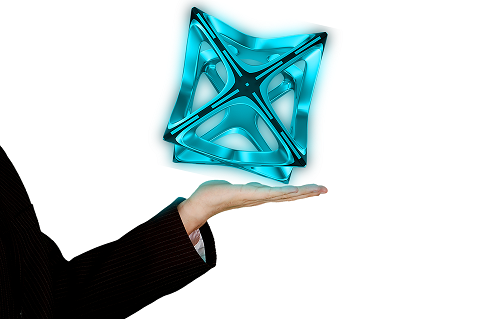
\includegraphics[width=0.8\linewidth]{images/hologram}
	\caption{Ein virtuell projizierter Hologramm-Würfel\cite{online4}}
	\label{fig:hologram}
\end{figure}


Die ersten Ansätze für eine mögliche Anwendung von der \textit{Augmented Reality} findet sich in der Literatur: In der Kurzgeschichte \textit{"Der Zauberer von Oz"} von L.Frank Baum wird nämlich eine Brille beschrieben, die dem Protagonist hilft Charaktereigenschaften von Figuren virtuell zu sehen.\cite{onlineAR} Erst Jahrzehnte später werden erste Augmented Reality Systeme getestet und schließlich der Begriff eingeführt. Es waren die Boeing-Mitarbeiter Tom Caudell und David Mizell die schließlich den Begriff Augmented Reality nutzten, um die Erweiterung der Realität mit virtuellen Informationen zu beschreiben.\cite{TomDavid}


\subsection{\label{sub2:thema}b.) Unsere eigene Definition von Augmented Reality}

Aus unserer Sicht umfasst die \textit{Augmented Reality} ...

\subsection{\label{sub3:thema}c.) Welche Ausprägungen und Abwandlungen gibt es?}

Augmented Reality kann vielseitig eingesetzt werden und wird mehr und mehr Teil des Alltags. In der Luft- und Raumfahrt z.B wird Augmented Reality schon lange benutzt. Es werden dort durch die Einblendung von Daten in ein Head-Up-Display wichtige Information für den Piloten bereitgestellt. Auch in der Industrie wird Augmented Reality im großen Stil eingesetzt. Sei es bei der Fertigung komplexer Bauteile oder im Flugzeug- und Autobau – über eine AR-Brille vermittelte Informationen zu komplexen Arbeitsschritten erleichtern häufig die Arbeit. Zunehmend wird Augmented Reality auch bei der Reparatur von Autos genutzt, da so Zeit gespart und Fehler vermieden werden. Auch in großen Lagerhallen wird den Gabelstaplerfahrern mithilfe von Augmented Reality Systemen Weginformation ins Sichtfeld eingeblendet. Häufig sind diese modernen Datenbrillen auch mit Lautsprechern ausgestattet, sodass die Nutzer nicht nur visuelle sondern auch auditive Hilfe bekommen. (siehe Abb. \ref{fig:autoholo})
\linebreak

\begin{figure}[H]
	\centering
	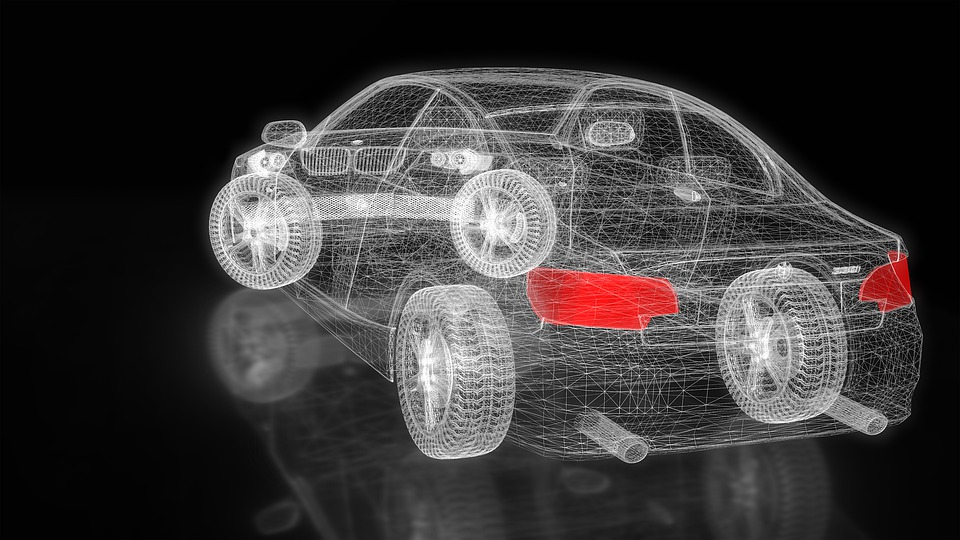
\includegraphics[width=0.8\linewidth]{images/autoholo}
	\caption{Heutzutage wird mithilfe von \textit{Augmented Reality} in der Automobil-Branche schon gearbeitet\cite{online5}}
	\label{fig:autoholo}
\end{figure}

Ein weiterer Bereich, für den \textit{Augmented Reality} zunehmend wichtiger wird, ist die Medizin.  Besonders minimal-invasive Eingriffe werden durch die Überblendung der betreffenden Körperstelle mit CT oder MRT Bildern erleichtert. Auch in Marketing und Verkauf wächst die Verwendung von Augmented Reality. So kann der Kunde beispielsweise virtuelle Kleidungsstücke anprobieren oder Möbelstücke vor dem Kauf virtuell an verschiedenen Stellen in der Wohnung platzieren. Auch am Point of Sale kann Augmented Reality rentabel sein, da der Kunde sich den Inhalt von Verpackungen mithilfe von Augmented Reality anzeigen lassen kann und somit einen dreidimensionalen Eindruck vom Produkt bekommt, ohne die Packung zu öffnen. Des Weiteren wird Augmented Reality gerne in der Unterhaltungs- und Spieleindustrie eingesetzt, da das Spielerlebnis so noch authentischer wird. Auch im Bereich Bildung werden erste Augmented Reality Anwendungen getestet – sei es um Schulkindern den Aufbau der Erde dreidimensional nahezubringen oder Medizinstudenten eine bessere Vorstellung des menschlichen Körpers zu vermitteln. (siehe Abb. \ref{fig:med})
\linebreak

\begin{figure}[H]
	\centering
	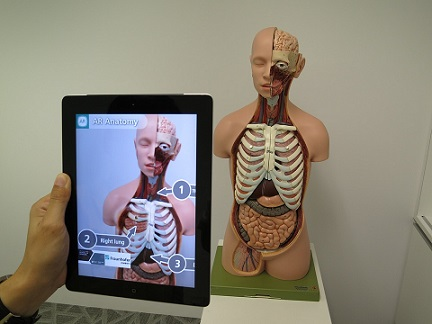
\includegraphics[width=0.8\linewidth]{images/medizin}
	\caption{In der Medizin wird \textit{Augmented Reality} auch schon verwendet} \cite{online3}
	\label{fig:med}
\end{figure}

\subsection{\label{sub4:thema}d.) Wie wird sich der Bereich in der Zukunft entwickeln?}

Durch die ständige Weiterentwicklung der Soft- und Hardware wird Augmented Reality immer größeren Nutzergruppen zugänglich. Durch die verbesserten technischen Gegebenheiten werden außerdem viele neue Anwendungen ermöglicht. Das englische Forschungsinstitut Juniper Research prognostiziert einen Zuwachs der Augmented-Reality-Nutzer von 60 Millionen im Jahr 2013 auf 200 Millionen im Jahr 2018. Tatsächlich wird Augmented Reality in vielen Bereichen immer stärker eingesetzt. So verwenden Unternehmen zunehmend AR, um ihre Produkte zu vermarkten und Kunden ein besseres Shoppingerlebnis zu ermöglichen. Beispiele hierfür sind die Screens von Lego, mit denen man einen dreidimensionalen Eindruck des Packungsinhalts bekommt oder der neue Ikeakatalog, den man als Marker nutzen kann, um beliebig virtuelle Möbel im eigenen Wohnraum auszuprobieren. Auch die Bedienung von PKWs ist dabei sich dahingehend zu verändern, dass man nicht mehr im Benutzerhandbuch nachlesen muss, sondern mit AR unterstützt wird. Langfristig ist auch die Erweiterung von Gesichtern mithilfe personenbezogener Information wie Kontaktdaten oder Details aus dem Lebenslauf denkbar, da Gesichtserkennungssysteme immer besser werden. Auch die Erkennung von Texten in einer fremden Sprache und die Erweiterung der Realität mit deren Übersetzung könnte in Zukunft möglich werden. Ein wichtiger Meilenstein in der Geschichte der Augmented Reality wird die Markteinführung der Google Glasses sein. Es handelt sich dabei um eine Brille, die verschiedenste Technologien nutzt, um die Realiät zu erweitern. Nicht alle Funktionen tracken die Realität, aber es bleibt abzuwarten, wie das fertige Produkt aussehen wird. (siehe Abb. \ref{fig:hologram})

\section{\label{sec:einfuehrung}Aufgabe 1.2: Unterschiede und Gemeinsamkeiten beim Verständnis von Wirtschaftsinformatik}
\subsection{\label{sub:einfuehrung}a.) Kriterien für einen Vergleich}

\begin{tabular}{|p{5cm}|p{10cm}|}
\hline
Kriterium & Erläuterung \\
\hline
Forschungsgegenstand & Forschungsgebenstand der Artikel. Bzw. die Hauptthemen mit welchen sich in der jeweiligen Zeitschrift beschäftigt wird.\\
\hline
Forschungsergebnisse & Art der Forschungsergebnisse der jeweiligen Zeitschrift. Also handelt es sich bei den Ergebnissen eher um Praxisrelevante Ergebnisse oder nur theoretische. \\
\hline
Praxisorientiertheit & Wie wichtig ist die Praxisorientiertheit der Artikel. Sind die Artikel im durchscnitt eher praxisorientiert oder ist dies eher nicht wichtig.\\
\hline
Forschungsmethoden & Bedeutung der Forschungsmethode für die Zeitschrift\\
\hline
Qualität / Bedeutung & Die Bedeutung der jeweiligen Zeitschrift im internationalen Vergleich zu anderen Zeitschrifften der gleichen Fachbereichs.\\
\hline
Zielgruppe & Die Zielgruppe welche von der jeweiligen Zeitschrift hauptsächich angesprochen wird. Also handelt es sich eher Personen aus der Wirtschaft wie Manager oder Facharbeiter oder Personen aus Forschung und Lehre.\\
\hline
\end{tabular}

\newpage
\subsection{\label{sub2:einfuehrung}b.) Vergleich von den Zeitschriften HMD und BISE}

\begin{tabular}{|p{4cm}|p{5.5cm}|p{5.5cm}|}
\hline
& HMD & BISE \\
\hline
Forschungsgegenstand & Entwicklung und verbesserung von Geschäftsprozessen und IS & Entwicklung und verbesserung von Geschäftsprozessen und IS \\
\hline
Forschungsergebnisse & praxisrelevante Ergebnisse & praxisrelevante Ergebnisse \\
\hline
Praxisorientierung & sehr wichtig & sehr wichtig \\
\hline
Forschungsmethoden & weniger wichtig & weniger wichtig \\
\hline
Qualität/ Wichtigkeit & international eher wenig bedeutend & international bedeutender \\
\hline
Zielgruppe & Fach- und Führungskräfte, Studierende und Lehrende (in Deutschland) & Fach- und Führungskräfte, Studierende und Lehrende (hauptsächlich in Deutschland und Europa) \\
\hline
\end{tabular}
\newline
\newline
\newline

Bei den beiden zu vergleichenden Zeitschriften \emph{HMD Praxis der Wirtschaftsinformatik} und \emph{BISE / WIRTSCHAFTSINFORMATIK} handelt es sich um Fachzeitschrifften aus dem Gebiet der Wirtschaftsinformatik. Bei beiden Zeitschriften handelt es sich um deutsche Veröffentlichungen. Wobei die \emph{BISE} seit 2015 nur noch in Englischer Sprache herausgebracht wird\cite{BISE}.

Sowohl die \emph{HMD} als auch die \emph{BISE} beschäftigen sich mit Herausforderungen und deren Lösungsideen sowie deren Umsetzungsmöglichkeiten\cite{Meier2017}\cite{Stein2017}\cite{Ebert2017}. Wie der Name der \emph{HMD Praxis der Wirtschaftsinformatik} schon sagt, sind die Ergebnisse aus Veröffent-lichungen sehr praxisrelevant. Dies trifft ebenfalls auf die \emph{BISE} zu. Artikel aus beiden Fachzeitschriften beziehen sich auf praktische Themen deren Praxistauglichkeit und teilweise auch wie diese wirklich umgesetzt werden können\cite{Meier2017}\cite{Stein2017}\cite{Ebert2017}\cite{Kakar2017}. Ein Beispiel für die Praxisorientiertheit der Zeitschriften ist der Artikel \emph{Spielerisch lockt der Einzelhandel den Kunden – Einfluss von Belohnungen auf die Kanalwahl}\cite{Stein2017} aus der \emph{HMD} von 2017. Er bezieht sich auf den Einsatz von Gamification im Einzelhandel und dessen Nutzen. 

Wenn es um die Bedeutung geht ist die \emph{HMD} internatilonal gesehen eine eher unbedeutende Zeitschrift (VHB-JOURQUAL-Ranking von D)\cite{VHBJ}. Allerdings wird sie auch hauptsächlich in Deutsch veröffentlicht. Daher ist sie auch hauptsächlich im deutschsprachigen Raum relevant. 
Die \emph{BISE} ist im Vergleich zur \emph{HMD} international schon deutlich relevanter (VHB-JOURQUAL-Ranking von B)\cite{VHBJ}. Allerdings ist sie trotz Veröffentli-chung in englischer Sprache, aufgrund der starken Neigung zur deutschen Wirtschaftsinformatik, vor allem in Europa relevant. 

Die Zielgruppe bei beiden Zeitschriften ist wieder ziemlich ähnlich. Beide Zeitschriften sind an Fach- und Führungskräfte sowie an Studierende und Lehrende gerichtet. Nur, dass die \emph{HMD} sich aufgrund der Sprache eher an den deutschsprachigen Raum und die \emph{BISE} ebenfalls an Englischsprachige richtet.
\newline
\newline

{\Large Fazit}

Inhaltlich sowie methodisch ähneln sich beide Zeitschriften sehr stark. Dies dürfte vor allem daran liegen, dass die \emph{HMD} und die \emph{BISE} sowohl aus dem selben Fachgebiet (Wirtschaftsinformatik) als auch aus der selben Region (Deutschland) kommen.
\subsection{\label{sub3:einfuehrung}c.) Vergleich von den Zeitschriften MISQE und ISR}

\begin{tabular}{|p{4cm}|p{5.5cm}|p{5.5cm}|}
\hline
& MISQE & ISR \\
\hline
Forschungsgegenstand & Wichtiges und Nützliches für die Praxis der Information Systems & Theorie und Hintergründe der Information Systems \\
\hline
Forschungsergebnisse & teils sehr Praxisnah & kaum Praxisbezug \\
\hline
Praxisorientierung & wichtig & teils vorhanden, teils nicht \\
\hline
Forschungsmethoden & wichtig & wichtig \\
\hline
Qualität/ Wichtigkeit & international eine wichtige und geschätzte Zeitschrift in dieser Fachrichtung & international eine der am meisten bedeutenden Zeitschriften dieser Fachrichtung \\
\hline
Zielgruppe & Manager und Investoren und andere Führungskräfte sowie Forschende & Forschende sowie Fach- und Führungskräfte \\
\hline
\end{tabular}
\newline
\newline
\newline

Das Journal \emph{Information Systems Research} gehört zu den führenden Zeitschriften in der Fachrichtung der \emph{Information Systems} und wird auf der ganzen Welt anerkannt. Das Journal \emph{MIS Quarterly Executive} ist eine Schwester Veröffentlichung von \emph{MISQ}\citep{MISQE}, ebenfalls eine der größten Fachzeitschriften im Gebiet der \emph{Information Systems}, ist selbst allerdings nicht ganz so anerkannt und gefragt, genießt aber dennoch einen relativ hohen Stellenwert.

Die beiden Journals unterscheiden sich grundlegend bezüglich ihrer Forschungsgegenstände. Während \emph{MISQE} darauf ausgelegt ist Wichtiges und Nützliches für die Praxis der Information Systems zu behandeln und erforschen\citep{MISQE}, behandelt die \emph{ISR} eher die Theorie und Hintergründe der Information Systems\citep{ISR}. Daraus folgt auch unweigerlich, dass die Ergebnisse, die \emph{MISQE} liefert, deutlich Praxisrelevanter sind, als Ergebnisse von \emph{ISR}. Die Artikel aus \emph{MISQE} gehen auf Probleme in der Wirtschaft ein und geben Gründe und Empfehlungen für diese an bzw. versuchen die Zukunftsfähigkeit zu beurteilen\citep{Chasin2017}\cite{Lacity2017}. Die Artikel aus der \emph{ISR} hingegen gehen vorwiegend auf die Hintergründe ein\cite{Karhu2018}\cite{Constantinides2018}.

Wie bereits in der Einleitung erwähnt sind beide Journals recht angesehen im Gebiet der Information Systems. Dies verdeutlicht auch das VHB-JOUQAL-Ranking der Wirtschaftsinformatik. Hier belegt \emph{ISR}, eine "herausragende, weltweit führende wissenschaftliche Zeitschrift"\ den ersten Rang mit einer Spitzennote von A+, während \emph{MISQE} immerhin noch ein B bekommt, also "nur"\ eine "wichtige und angesehene wissenschaftliche Zeitschrift"\ ist\cite{VHBJ}.

Auch in der Zielgruppe unterscheiden sich beide Journals leicht. Während sich \emph{MISQE} aufgrund der starken Praxisorientierung eher an Manager, Investoren und andere Führungskräfte\citep{Chasin2017}\citep{MISQE} wendet und nur sekundär an die Forschung, ist es bei \emph{ISR} genau anders herum. Aufgrund der eher theoretischen Ergebnisse ist dieses Journal eher in der Forschung relevant\citep{ISR}. 
\newline

{\Large Fazit}

Zwischen \emph{MISQE} und \emph{ISR} gibt es doch einige bedeutende Unterschiede. Während \emph{MISQE} eher Praxisorientiert ist, konzentriert sich \emph{ISR} auf die Theorie. Allerdings sind beide Journals anerkannt und weltweit verbreitet. 



\subsection{\label{sub4:einfuehrung}d.) Vergleich von den Veröffentlichungen aus Deutschland (HMD und BISE) mit denen aus dem internationalen bzw. anglo-amerikanischen Bereich (MISQE und ISR).}

\begin{tabular}{|p{4cm}|p{5.5cm}|p{5.5cm}|}
\hline
& HMD und BISE & MISQE und ISR \\
\hline
Forschungsgegenstand & Entwicklung und Verbesserung von Geschäftsprozessen und IS & Teils Praxis, teils Theorie von Information Systems \\
\hline
Forschungsergebnisse & praxisrelevante Ergebnisse & teils sehr praxisnah, teils kaum Praxisbezug \\
\hline
Praxisorientierung & sehr wichtig & teils wichtig, teils nicht \\
\hline
Forschungsmethoden & weniger wichtig & wichtig \\
\hline
Qualität/ Wichtigkeit & international nur teilweise bedeutend & international zwei der am meisten bedeutenden Zeitschriften dieser Fachrichtung \\
\hline
Zielgruppe & Fach- und Führungskräfte, Studierende und Lehrende (größtenteils in Deutschland) & Forschende sowie Fach- und Führungskräfte (weltweit) \\
\hline
\end{tabular}
\newline
\newline
\newline

Vergleicht man die Veröffentlichungen aus Deutschland mit denen aus dem internationalen Raum, fällt einem sofort die unterschiedliche Bedeutung der Journals auf. Während die rein deutschsprachige Zeitschrift \emph{HMD} international so gut wie keine Bedeutung hat, gelten \emph{ISR} und \emph{MISQE} als absolut anerkannt in ihrer Branche. Sie sprechen Forschende, Führungskräfte und weiteres Fachpersonal auf der ganzen Welt an, während Zeitschriften wie \emph{BISE} allemal in Europa eine Bedeutung haben\cite{VHBJ}. 

Man erkennt allerdings auch, dass sich die beiden in Deutschland erscheinenden Zeitschriften in ihrer Form sehr ähneln, während es bei den internationalen Zeitschriften große Unterschiede gibt. Die \emph{MISQE} ähnelt eher einer Zeitschrift der Wirtschaftsinformatik, da sie  sich mit sehr praxisnahen Themen beschäftigt und auch praxisrelevante Ergebnisse erzielt. Die \emph{ISR} hingegen erinnert eher an Information Systems, da sie sich größtenteils mit der Theorie und den Hintergründen beschäftigt. Sie liefert so gut wie keine praxisnahen Ergebnisse. 
\newline

{\Large Fazit}

Zusammenfassend könnte man also sagen, dass \emph{MISQE} den deutschen Zeitschriften ähnelt, allerdings deutlich mehr Reichweite hat und deutlich anerkannter ist. \emph{ISR} hingegen ist eine Zeitschrift, die eher typisch für Information Systems ist.

\section{\label{sec:bonus}Bonusaufgabe}

Als Inspiration und Vorlage diente uns ein Stellenangebot auf \href{https://www.absolventa.de/stellenangebote/289852-p-junior-it-consultant-m-w-business-intelligence#external-job-offer}{www.absolventa.de}.\cite{online1} Mithilfe der Vorlage haben wir unser eigenes Stellenausschreiben geschrieben und geformt, wobei wir uns an der Struktur der Vorlage orientiert haben. Für das Design haben wir uns selber was einfallen lassen, z.B das Firmenlogo haben wir mit Paint selber erstellt und Icons als grafische Elemente verwendet, welche wir uns von einer No Copyright-Plattform für Bilder und Videos geholt haben.\cite{online2} Als Firmenname haben wir den Anfangsbuchstaben unserer Nachnahmen genommen. Auf der nächsten Seite ist das Stellenschreiben:

\newpage
\begin{figure}[htbp]
	\begin{minipage}[t]{4cm}
		\vspace{0pt}
		\centering
		
\includegraphics{images/Logo}
		\label{fig:Logo}
	\end{minipage}
	\hfill
	\begin{minipage}[t]{4cm}
		\vspace{0pt}
		\scriptsize
		\textbf{DSW \& Partner}\\
		Mr. Mustermann\\
		Personalleiter\\
		Bremen\\
		28195 Bremen\\
		Tel. +49 123 5160900 \\
		E-Mail: bewerbungen@dsw-partner.de
	\end{minipage}
\end{figure}

\large
\begin{center} Teamleiter im IT-Support\\(m/w/divers)\end{center} 

\scriptsize
Wir, das führende IT-Systemhaus in Bremen, suchen Dich als einen unserer neuen Teamleiter im IT-Support bei einen unserer vielen Kunden. In deinen Tätigkeiten als Teamleiter stehst du in der Aufgabe bei einen unserer Kunden ein Team effizient zu koordinieren, welche sämtliche Support-Funktionen,Aufgaben und Prozesse des Kunden übernimmt. Dich erwartet ein Team aus Informatikern im Bereich System- und Netzwerkadministration, Programmierung und weiteren IT-Profis. In unseren firmeninternen Weiterbildungsseminaren unserer DSW-Academy helfen wir dir deine technischen und sozialen Kompetenzen weiter zu entwickeln, sodass du ohne große Probleme dein Team führen kannst. Ob Partnerprogramm, einen eigenen Firmenwagen um flexibel zu sein oder Home Office – wir bieten Dir das Arbeitsumfeld, das Du für Deine persönliche Entwicklung benötigst.


\textbf{\\Deine Tätigkeiten bei uns sind:}
\begin{center}
	\begin{itemize}
		\item Für die Strukturierung und Koordination des IT-Support Teams zuständig
		\item Die fachliche Leitung und Weiterentwicklung des IT-Support Teams
		\item Optimierung von Prozessen und Abläufen 
		\item Sicherstellung und Steuerung der Anwenderbetreuung
		\item Übernahme von kundenbezogenen IT-Projekten
	\end{itemize}
\end{center}

\textbf{\\Deine Qualifikationen:}
\begin{center}
	\begin{itemize}
		\item Abgeschlossenes Studium der (Wirtschafts-) Informatik oder vergleichbare Ausbildung
		\item Du hast bereits mehrjährige Berufserfahrung im IT Bereich
		\item Du bringst Erfahrungen im Führen von Mitarbeitern
		\item Du hast Freude daran, zusammen mit unseren Kunden individuelle Lösungen zu entwickeln und diese anschließend zu implementieren
		\item Du hast Spaß an der Zusammenarbeit im Team und bist reisebereit
	\end{itemize}
\end{center}

\begin{center}
	\textbf{Deine Vorteile bei uns:}
\end{center}

\begin{center}
	
\includegraphics{images/auto}\label{fig:auto}\hspace{1,5cm}
	
\includegraphics{images/home}\label{fig:home}\hspace{1,5cm}	
	
\includegraphics{images/handshake}\label{fig:handshake}\hspace{1,5cm}		
	
\includegraphics{images/statistics}\label{fig:statistics}  
\end{center}
\hspace{0,3cm}\textbf{Eigener Firmenwagen,\hspace{0,7cm} Flexibel sein durch \hspace{0,9cm}Partnerschaftliches \hspace{1,1cm}Gute Karriere- \& \\ \hspace{0,4cm}auch Privat nutzbar\hspace{1,5cm}Home Office\hspace{2,1cm}Verhältniss \hspace{2cm}Aufstiegschancen} 			

\vspace{1cm}
\textbf{Wir haben dein Interesse geweckt?}\\
Schreib uns deine Bewerbung direkt per Email an die oben genannte Adresse oder bewirb Dich online über: www.dombeck-schwarz-warnke/DSW-partner/stellenangebote/.de – Das Stellenangebot findest du unter der Rubrik 'IT Support'.

\normalsize
\newpage
\addcontentsline{toc}{section}{Literaturverzeichniss}
\bibliography{Literaturdatenbank}

\end{flushleft}
\end{document}
